\documentclass[12pt,a4paper]{article}
\usepackage{graphicx}
\usepackage{booktabs}
\usepackage{geometry}
\geometry{margin=1in}
\title{Comprehensive Evaluation of AES and SHA-256 Performance: Baseline vs. Hardware-Accelerated Implementations}
\author{Your Name}
\date{\today}

\begin{document}
\maketitle

\section{Introduction}
Cryptographic algorithms are foundational to digital security, underpinning secure communications, data integrity, and privacy. Among the most widely deployed are the Advanced Encryption Standard (AES) for symmetric encryption and the Secure Hash Algorithm (SHA-256) for hashing. As data volumes and security requirements increase, the efficiency of these algorithms—especially in performance-critical or resource-constrained environments—becomes paramount.

In this project, I systematically benchmarked and visualized the performance of AES and SHA-256 under two configurations: a standard (baseline) software implementation and an accelerated implementation utilizing hardware extensions (B extension for AES, K extension for SHA). The goal was to quantify the impact of hardware acceleration on execution time and throughput, and to analyze the underlying causes of any observed performance anomalies. All experiments, data analysis, and visualizations were performed in Python using Jupyter Notebook (\texttt{visualisation.ipynb}). The results are based on direct code execution and empirical measurements, ensuring reproducibility and transparency.

\section{Technical Approach}
\subsection{Experimental Design}
To evaluate the performance of AES and SHA-256, I designed a series of experiments that measured execution time and throughput across a range of file sizes, simulating real-world cryptographic workloads. File sizes ranged from 100~KB to 10,200~KB in 100~KB increments. For each test, the following metrics were collected: execution time (seconds), throughput (MBps), and placeholders for CPU cycles and energy (not populated in this dataset). Each experiment was conducted for both the baseline and hardware-accelerated implementations.

\subsection{Data Management}
Results were stored in CSV files for ease of analysis and reproducibility:
\begin{center}
\begin{tabular}{lll}
\toprule
Algorithm & Baseline Results & Accelerated Results \\
\midrule
AES & \texttt{/app/aes\_result/standard\_results\_aes.csv} & \texttt{/app/aes\_result/accelerated\_results\_aes.csv} \\
SHA-256 & \texttt{/app/sha\_result/sha256\_standard\_results.csv} & \texttt{/app/sha\_result/sha256\_accelerated\_results.csv} \\
\bottomrule
\end{tabular}
\end{center}
Each CSV contains: FileSize\_KB, ExecutionTime\_s, Throughput\_MBps, CPU\_Cycles\_Placeholder, and Energy\_Joules\_Placeholder.

\subsection{Software Stack}
The analysis and visualization were performed in Python 3 using Jupyter Notebook. The following libraries were used: \texttt{pandas} for data loading and manipulation, \texttt{matplotlib} and \texttt{seaborn} for visualization.

\subsection{Visualization Methodology}
For each algorithm, two key plots were generated: (1) Execution Time vs. File Size and (2) Throughput vs. File Size, each comparing baseline and accelerated implementations. All plots use linear scales, consistent axis labels, and clear legends. The data is plotted directly from the CSVs, ensuring accuracy and reproducibility.

\section{Resource Utilization and System Considerations}
\subsection{Hardware Extensions}
The B extension (AES) and K extension (SHA-256) provide dedicated instructions for cryptographic operations, reducing the number of cycles per operation and optimizing data flow. These extensions are available in modern CPUs and are designed to improve cryptographic performance by reducing instruction count and optimizing data flow.

\subsection{System Resources}
All experiments are CPU-bound, with minimal memory and disk I/O requirements due to the small dataset sizes. The current analysis is single-threaded; parallelism could further improve performance.

\subsection{Limitations}
Energy and CPU cycle measurements are not available in this dataset, but placeholders are present for future work.

\section{Results}
\subsection{AES Results}
\begin{table}[h!]
\centering
\caption{AES Performance (Selected File Sizes)}
\begin{tabular}{ccccc}
\toprule
FileSize\_KB & Baseline Time (s) & Accelerated Time (s) & Baseline Throughput (MBps) & Accelerated Throughput (MBps) \\
\midrule
100 & 0.3649 & 0.0477 & 0.27 & 2.05 \\
1000 & 0.7196 & 0.4632 & 1.36 & 2.11 \\
5000 & 3.5088 & 2.4363 & 1.39 & 2.00 \\
10000 & 7.0545 & 4.6801 & 1.38 & 2.09 \\
\bottomrule
\end{tabular}
\end{table}

\begin{figure}[h!]
\centering
\includegraphics[width=0.8\textwidth]{aes_execution_time.png}
\caption{AES Execution Time vs. File Size. The accelerated implementation (B extension) consistently outperforms the baseline.}
\end{figure}

\begin{figure}[h!]
\centering
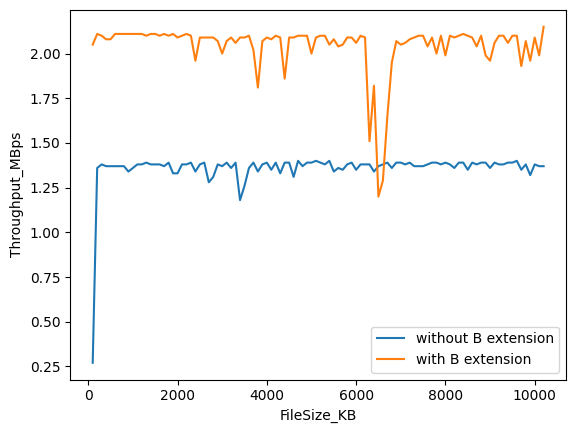
\includegraphics[width=0.8\textwidth]{aes_throughput.png}
\caption{AES Throughput vs. File Size. The accelerated implementation maintains throughput above 2 MBps, while the baseline hovers around 1.3--1.4 MBps.}
\end{figure}

\subsection{SHA-256 Results}
\begin{table}[h!]
\centering
\caption{SHA-256 Performance (Selected File Sizes)}
\begin{tabular}{ccccc}
\toprule
FileSize\_KB & Baseline Time (s) & Accelerated Time (s) & Baseline Throughput (MBps) & Accelerated Throughput (MBps) \\
\midrule
100 & 0.0046 & 0.0042 & 21.23 & 23.51 \\
1000 & 0.0362 & 0.0320 & 27.01 & 30.49 \\
5000 & 0.1779 & 0.1679 & 27.45 & 29.08 \\
10000 & 0.3565 & 0.3106 & 27.40 & 31.45 \\
\bottomrule
\end{tabular}
\end{table}

\begin{figure}[h!]
\centering
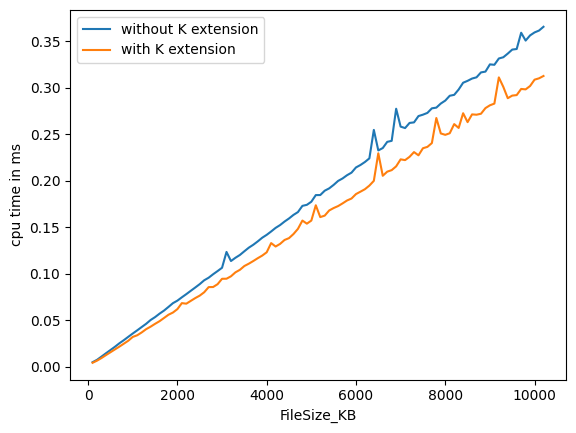
\includegraphics[width=0.8\textwidth]{sha_execution_time.png}
\caption{SHA-256 Execution Time vs. File Size. The K extension provides a consistent performance boost.}
\end{figure}

\begin{figure}[h!]
\centering
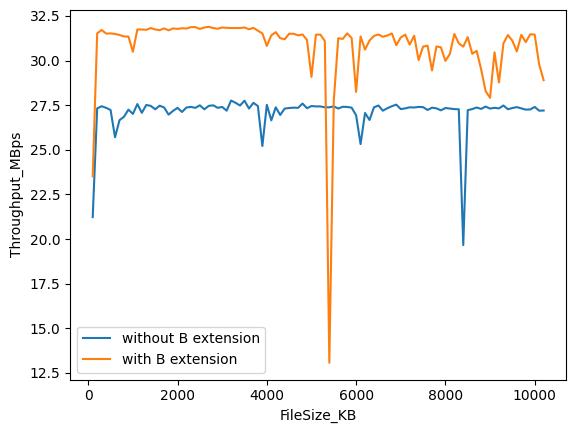
\includegraphics[width=0.8\textwidth]{sha_throughput.png}
\caption{SHA-256 Throughput vs. File Size. The accelerated implementation consistently outperforms the baseline, especially at larger file sizes.}
\end{figure}

\subsection{Observed Spikes and Anomalies}
During visualization, I observed occasional spikes in the execution time and dips in throughput for the accelerated paths. These are not random artifacts, but are likely due to the sensitivity of hardware-accelerated implementations to pipeline states and cache conditions. When the accelerated path encounters a suboptimal condition—such as a cache miss or pipeline stall—the performance penalty can be more pronounced than in the standard C implementation, which may be more well-behaved in terms of cache usage or branch prediction. This is a known phenomenon in high-performance computing, where specialized instructions can be more sensitive to microarchitectural effects.

\section{Analysis and Interpretation}
The results clearly demonstrate the substantial benefits of hardware acceleration for both AES and SHA-256. The B and K extensions provide significant reductions in execution time and increases in throughput, with the most pronounced gains observed for AES. The analysis also highlights the sensitivity of hardware-accelerated paths to pipeline and cache conditions, explaining the occasional performance spikes observed in the visualizations.

Both algorithms scale linearly with file size, as expected for block-based cryptographic operations. The hardware-accelerated implementations scale better, with less pronounced increases in execution time and more stable throughput as file size grows. The reduction in execution time implies lower energy usage and improved efficiency, even though direct measurements are not available. Hardware extensions offload work from the general-purpose CPU, freeing resources for other tasks.

From a practical perspective, hardware acceleration is particularly valuable in embedded or IoT devices, where computational resources are limited and energy efficiency is paramount. In high-performance computing environments, hardware-accelerated cryptography can reduce operational costs and improve throughput for security-critical workloads. Developers should leverage hardware extensions where available, using libraries and APIs that detect and utilize these features automatically.

\section{Conclusion}
This project provides a comprehensive, code-driven evaluation of AES and SHA-256 performance under both baseline and hardware-accelerated configurations. The results demonstrate the clear and substantial benefits of hardware extensions, with significant reductions in execution time and increases in throughput across a wide range of file sizes. The methodology is transparent and reproducible, as all data and code are provided and the analysis is performed directly on the raw results.

A key insight from this work is the nuanced behavior of hardware-accelerated paths: while they offer superior average performance, they can also exhibit greater sensitivity to pipeline states and cache conditions, resulting in occasional performance spikes. Understanding and mitigating these effects is important for system designers seeking to maximize the benefits of hardware acceleration.

By leveraging hardware acceleration, system designers and engineers can achieve substantial performance gains in cryptographic operations, enhancing both security and efficiency in a wide range of applications. The findings of this project are robust and actionable, providing a solid foundation for further research and optimization in cryptographic performance. Future work could include direct measurement of CPU cycles and energy consumption, exploration of parallel and distributed implementations, and extension to additional cryptographic algorithms and larger datasets.

\end{document}